\chapter{Parameterization}
\label{parameterization}
\section{Background}
Aerodynamics shape optimization (ASO) is the process that involves optimizing an aero-shape (wing, airfoil, fuselage, so on) under given constraints. The objective function can be drag, lift, aerodynamic efficiency, and so on. Representing the wing requires a tedious job of plotting the actual surface. The wing surface is to be parameterized using parameterization schemes. There are multiple ways to parametrize the wing, which include mesh-points, B-splines, cubic splines, free-form deformation. Representing the wing using the parameterization reduces the dimension of the design space. 

A shape parameterization system typically involves the coupling of a CAD tool and a grid generator. Every time the shape design variables are changed, a new grid must get generated without human intervention. For complex problems and especially involving RANS models, fully automatic grid generation can be difficult or impossible. An alternative approach is to use a reference shape, usually the starting design, and deform this shape by various techniques. In the present work, the FFD parameterization technique is selected because it is easy to implement and gives more flexibility while perturbating control points. The subsequent sections cover the detailed approached on FFD.

\section{Problem statement}
Before discussing the parameterization and construction of the wing, the problem statement and constraints will be discussed initially.

The objective is to minimize $C_d$, subject to constraints as mentioned.
\begin{frame}{\underline{Problem statement}}
\section{Problem statement}
\small{To solve the ADO-DG  (\textit{Aerodynamic Design Optimization and Discussion Group}) case 6: }
\\[2mm]
\begin{itemize}
\item Objective function is to minimize $C_D$
\item $C_L$ = 0.375, Mach = 0.5
\item Baseline geometry NACA 0012 wing with semi span 3.06 units
\item  Intented to have multimodal optima
\item Geometric parameters as described in the problem
\end{itemize}

\parbox{0.38\linewidth}{
\textit\textit{{Result should highlight:}}
\begin{itemize}
\item Number of optima 
\item Geometry description of each optimal wing
\item Evidence for convergence
\item Performance value, $eb^2$, b as final span, and $e$(span efficiency factor) is defined as,
$$\boxed{
e=\frac{C_{L}^{2}}{2 \pi S C_{D}}
}$$
\end{itemize}
}
\parbox{0.57\linewidth}{
\begin{figure}
    \centering
    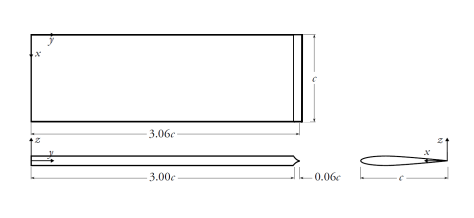
\includegraphics[scale = 0.34]{figures/baselinewing.png}
    \caption{baseline wing}
    \label{fig:baseline wing}
\end{figure}
}

\end{frame}

The AoA and $C_l$ constraint are satisfied by the CFD solver (SU2). The root bending moment ($C_{M_x}$) constraint is implemented into the Python code using feasibility rules proposed by Deb and Saha \cite{Deb}. The shape constraints like thickness, chord, semi span of a wing are satisfied using the Python code coupled with FFD control points displacement, which will be discussed in further sections.

\section{Free Form Deformation}
FFD is a process by which shape change can be made to geometry by manipulating the location of points which are related to the geometry. Soderberg and Parry first introduced this technique in 1986. It can be correlated to the Bezier curves of parameterization of given curves. Before going directly with wing parameterization, a short introduction on the FFD applied to 2D geometries will be presented.

As mentioned before, FFD manipulates the geometry by attaching it to bezier curves. And these curves are defined by the grid of control points defined as $u \in[0,1]$, $t\in[0,1]$.The Bernstein polynomials govern the control points' influence on the space within the grid. The effect of perturbation reduces with the distance between mesh points from the control point. However, it is observed that moving the control points within the grid will have less effects. Figure \ref{ffd_effect} represents the same.

\begin{figure}
    \centering
    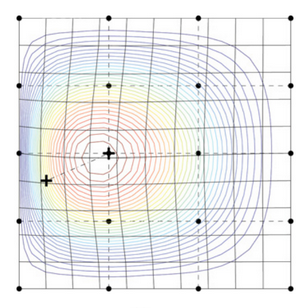
\includegraphics[scale=0.56]{figures/ffd5.png}
    \caption{FFD control point grid with the a(2,3) control point displaced. The solid lined grid show how mesh points are shifted according to the influence of the control points\cite{ffd_book}.}
    \label{ffd_effect}
\end{figure}

Equation \ref{ffd_2d} represents the mathematically form of 2-D FFD box.
\begin{equation}
\mathbf{X}(u, t)=\sum_{i=0}^{n} \sum_{j=0}^{m} \mathbf{a}^{(i, j)} f_{i}(u) g_{j}(t)
\label{ffd_2d}
\end{equation}

where \textbf{X}(u, t) is the Cartesian coordinates of the new, deformed location of a point at (u, t). And, $f_i(u)g_j(t)$ represents the Bernstein polynomial, $a^{(j,i)}$ represent the control point being displaced. To make this work, define a shape in parametric form and apply equation \ref{ffd_2d}. However, care should be taken to inscribe the entire object, subjected to deformation, into the FFD box; else, only the inscribed part will be deformed.

Extending further, same concept can be implemented to 3D problems. Every object point \textbf{X} has (s,t,u) coordinates in the parallelpiped coordinate region\cite{soderberg}.

\begin{equation}
\mathbf{X}=\mathbf{X}_{0}+s \mathbf{S}+t \mathbf{T}+u \mathbf{U}
\label{ffd initial equation}
\end{equation}

Let $\textbf{P}_{ijk}$, i = 0, \dots, l, j = 0,\dots, m, k = 0,\dots, n are control points on the lattice. Equation \ref{ffd_3d} represents the mathematical form of 3D FFD box equation.
\begin{equation}
\mathbf{X}(u, t, s)=\sum_{i=0}^{m} \sum_{j=0}^{n} \sum_{k=0}^{p} \mathbf{a}^{(i, j, k)} f_{i}^{m}(u) g_{j}^{n}(t) h_{k}^{p}(s)
\label{ffd_3d}
\end{equation}
where Bernstein's polynomial $f_{i}^{m}(u)$ is defined as,

\begin{equation}
f_{i}^{m}(u)=\frac{(m) !}{(i) !(m-i) !} u^{i}(1-u)^{m-i}
\label{bernstein_poly}
\end{equation}

The new position of a point $\textbf{X}_{def}$ is computed by:

\begin{equation*}
\mathbf{X}_{d e f}=\sum_{i=0}^{l}\left(\begin{array}{l}
l \\
i
\end{array}\right)(1-s)^{l-i} s^{i}\left[\sum_{j=0}^{m}\left(\begin{array}{c}
m \\
j
\end{array}\right)(1-t)^{m-j} t^{j}\left(\sum_{k=0}^{n}\left(\begin{array}{l}
n \\
k
\end{array}\right)(1-u)^{n-k} u^{k} \mathbf{P}_{i j k}\right)\right]\end{equation*}

As compared to 2D FFD equation, 3D FFD requires an additional set of Bernstein's polynomial and a 3D grid points. Figure \ref{sphere_ffd} illustrates the influence of the control point movement on the sphere, when one of the control points is displaced away. Similarly, another example mentioned in figure \ref{wing_ffd} represents the wing shape deformation (preciously surface mesh deformation) due to wingtip control points being rotated and translated.

\begin{figure}
\parbox{0.49\linewidth}
{
\centering
 \framebox{ 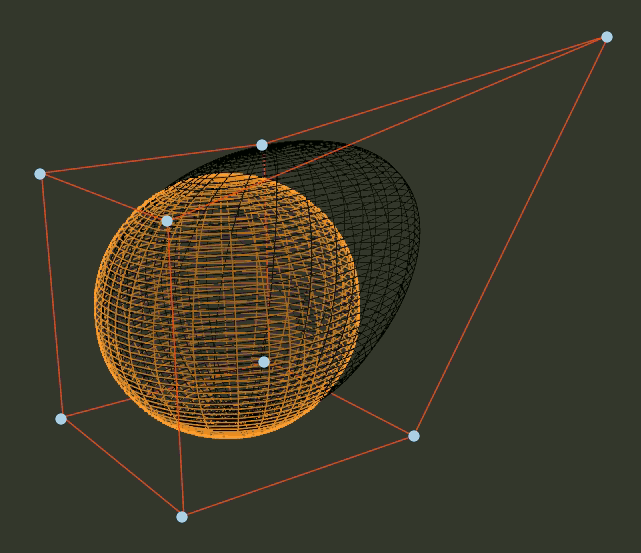
\includegraphics[width = 65mm,height = 65mm]{figures/sphere_ffd.png} }
 \caption{Influence of the control point over the sphere body with $a^{(m,n,p)}$ as $2 \times 2 \times 2$ control points.}
 \label{sphere_ffd}
}
\parbox{0.47\linewidth}
{
\centering
  \framebox{  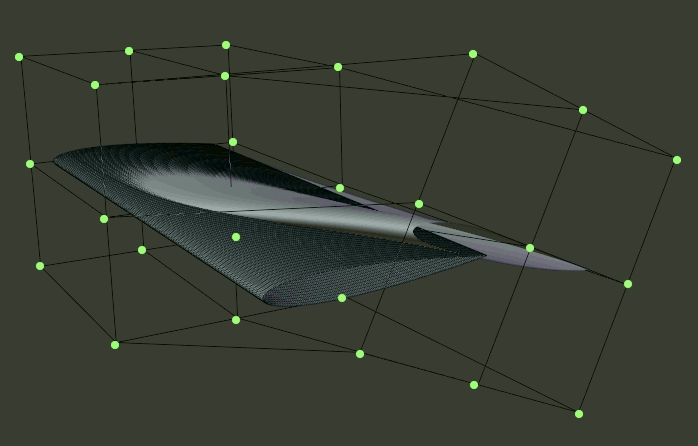
\includegraphics[width = 65mm,height = 65mm]{figures/ffd_wing.png}}
  \caption{FFD of a wing shape, with the control points on the face of the wing-tip end are rotated and translated.}
  \label{wing_ffd}
}
\end{figure}

In figure \ref{wing_ffd}, the wing surface mesh is parameterized using the FFD with 27 control points. However, this work contains 60 control points to deform a wing surface mesh. Full details about the distribution of control points will be explained in the upcoming chapter. Figure \ref{wing1_span} to \ref{wing3_iso} represents the perturbed wing which are obtained after implementing FFD box and perturbing the control points of FFD box.

\begin{figure}[!ht]
    \parbox{0.47\linewidth}
    {
    \centering
    \framebox{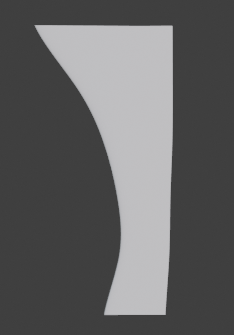
\includegraphics[width = 65mm,height = 65mm]{figures/wing2_span.png}}
    \caption{Span view of wing 1.}
    \label{wing1_span}
    }
    \parbox{0.47\linewidth}
    {
    \centering
    \framebox{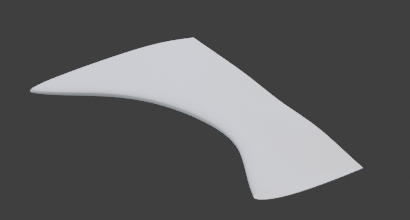
\includegraphics[width = 65mm,height = 65mm]{figures/wing2_iso.png}}
    \caption{Iso view of wing 1.}
    \label{wing1_iso}
    }
\end{figure}


\begin{figure}[!ht]
    \parbox{0.47\linewidth}
    {
    \centering
    \framebox{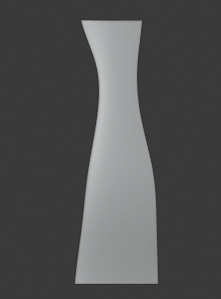
\includegraphics[width = 65mm,height = 65mm]{figures/wing6_span.png}}
    \caption{Span view of wing 2.}
    \label{wing2_span}
    }
    \parbox{0.47\linewidth}
    {
    \centering
    \framebox{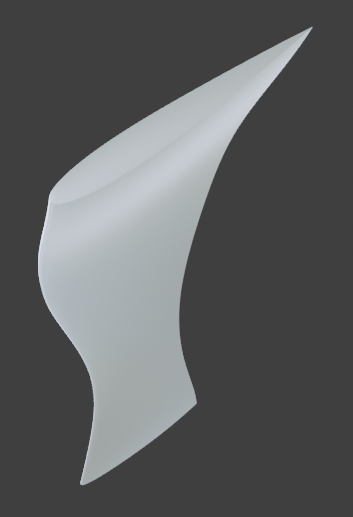
\includegraphics[width = 65mm,height = 65mm]{figures/wing6_iso.png}}
    \caption{Iso view of wing 2.}
    \label{wing2_iso}
    }
\end{figure}


\begin{figure}[!ht]
    \parbox{0.47\linewidth}
    {
    \centering
    \framebox{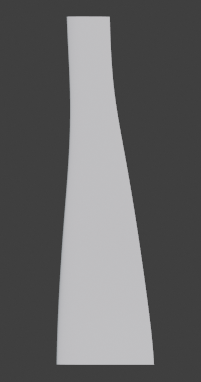
\includegraphics[width = 65mm,height = 65mm]{figures/wing3_span.png}}
    \caption{Span view of wing 3.}
    \label{wing3_span}
    }
    \parbox{0.47\linewidth}
    {
    \centering
    \framebox{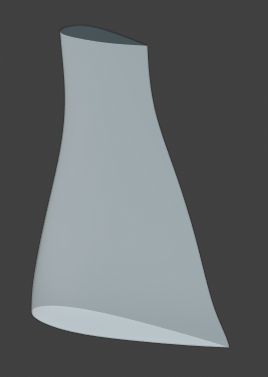
\includegraphics[width = 65mm,height = 65mm]{figures/wing3_iso.png}}
    \caption{Iso view of wing 3.}
    \label{wing3_iso}
    }
\end{figure}
\section{FFD implementation algorithm}
Evaluation and implementation of the FFD equation are explained in the algorithm \ref{ffd_algorithm}. Input to this algorithm will be parametric coordinates of object surface mesh. Output of the algorithm will be the cartesian coordinates of deformed surface mesh.
\begin{algorithm}
\SetAlgoNoLine
\textbf{Input}: parameters (s,t,u)\\
\textbf{Output}: new coordinates of the point \textbf{X} for parameters (s,t,u)\\
  \For{i=0, \dots , l}
  {
    \For{j=0, \dots , m}
    {
        \For{k=0, \dots , n}
        {
        $X=X+\operatorname{binom}(l, i) * \operatorname{pow}(1-s, l-i) * \operatorname{pow}(s, i) *$
$\operatorname{binom}(m-1, j) * \operatorname{pow}(1-t, m-j) * \operatorname{pow}(t, j) *$
$\operatorname{binom}(n, k) * \operatorname{pow}(1-u, n-k) * \operatorname{pow}(u, k) * \boldsymbol{P}_{i j k}$
        }
    }
  }
 \caption{FFD algorithm}
 \label{ffd_algorithm}
\end{algorithm}

Note that function $binom$ is the computation of binomial number and function $pow(a, b)$ is power $a^b$.

\section{Reduced-order model}
After considering the effort involved in building the FFD box, the next issue to address is the algorithm's credibility over solving the higher dimension problem. At present, the problem dimension is 125. The DE based niching algorithm is not tested for the 125 dimension problem, resulting in reconsider to reduce the problem dimension. The preferred way to carry out the dimension reduction is reduced-order modeling.

Complex geometries encountered in aerodynamics typically require a large number of grid points to define the surface boundaries. For example, the representation of the standard wing involves a million+ grid points. Apart from this, if the number of random input variables (geometry variables) is not restricted, then the computational cost would increase linearly. Figure \ref{comp_power} represents the time taken by the algorithm versus the dimension of the problem. The time taken by the algorithm increases linearly with the dimension of the problem.

\begin{figure}[!htbp]
    \centering
    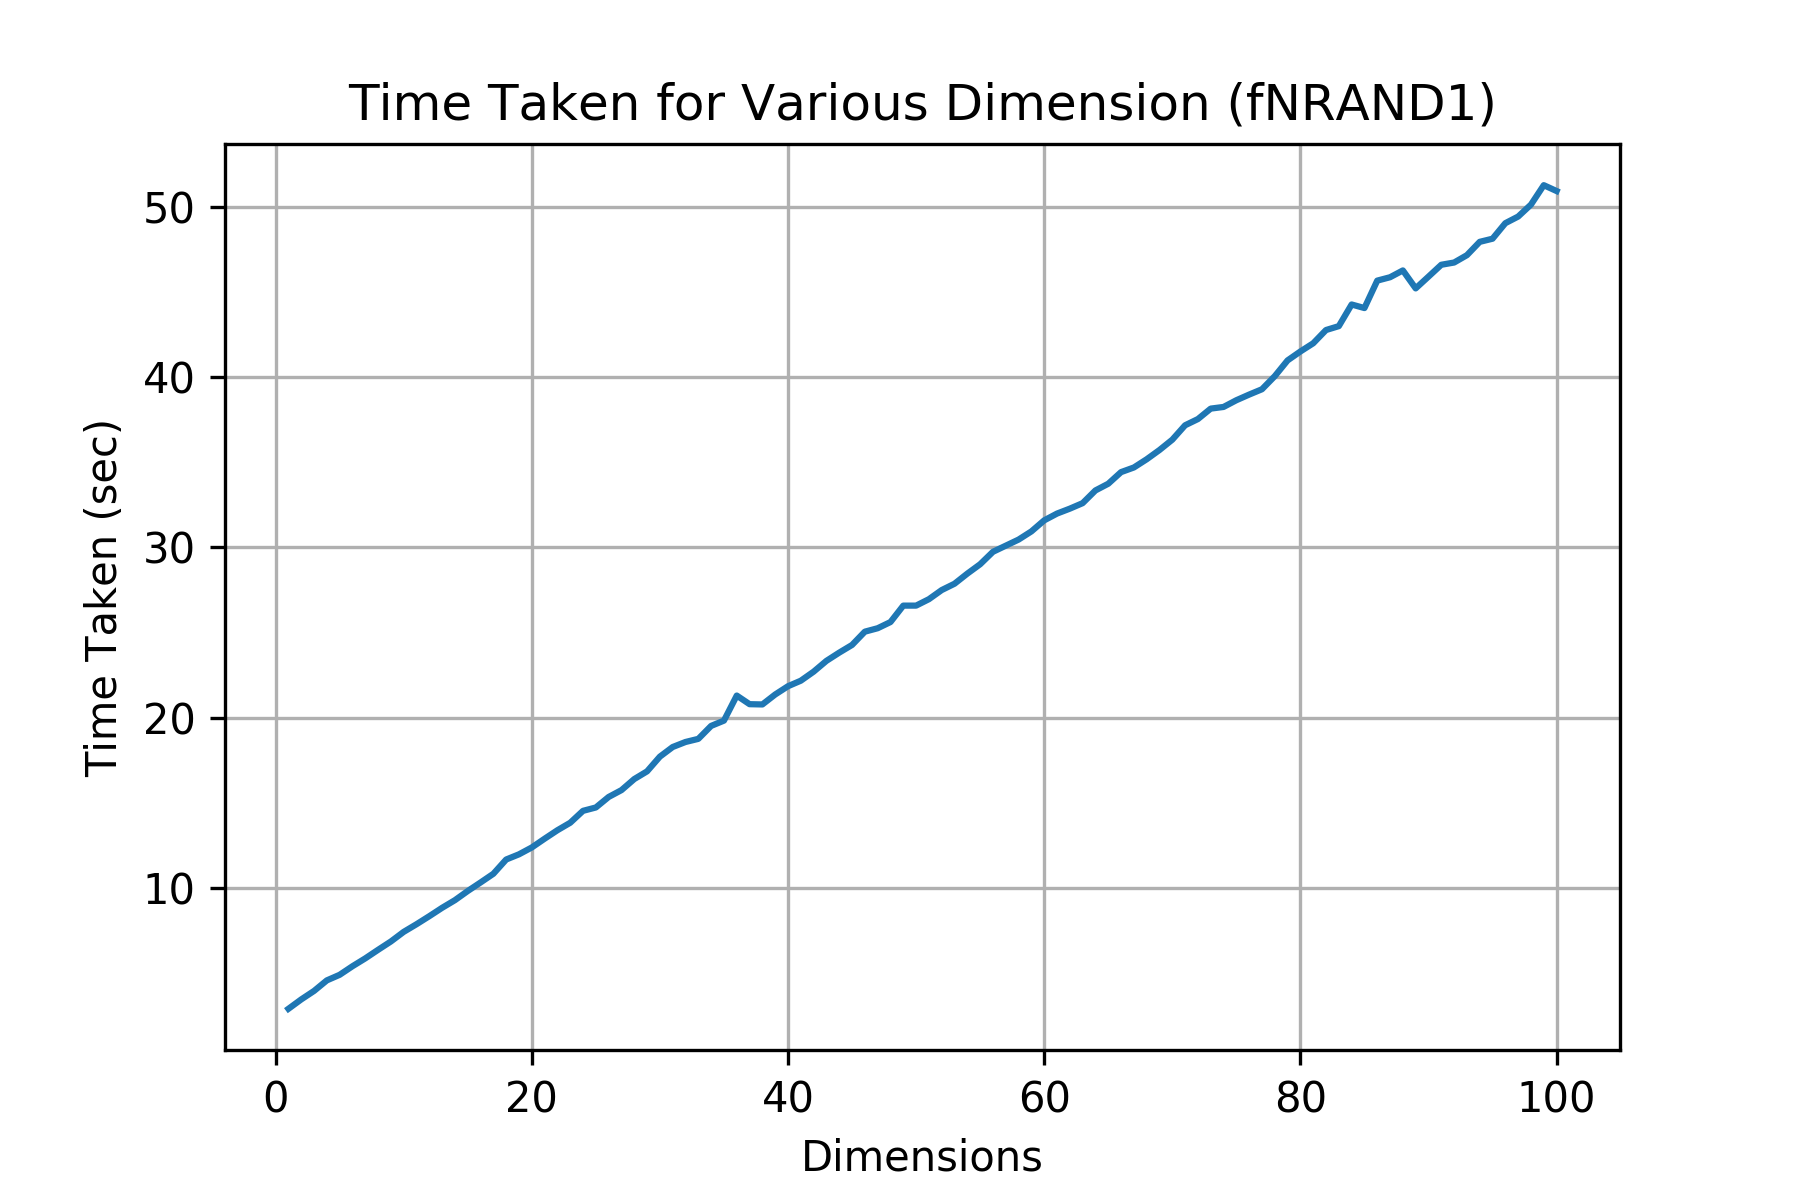
\includegraphics[width = \textwidth, height=85mm]{figures/plot_dimension_time_taken.png}
    \caption{Computational power varies linearly with dimension.}
    \label{comp_power}
\end{figure}

To reduce the additional computational cost, reduced-order modeling of the geometry is necessary. Once the dimension of problem is reduced to a manageable level, optimization of the NACA0012 wing can be implemented.

Reduced-order modeling is a highly complex topic and has found many applications in various fields of engineering. Typically reduced-order modeling methods can be categorized as parametric and non-parametric.

Parametric methods require a priori knowledge about the system to be reduced, whereas the non-parametric does not require any prior knowledge of the geometric uncertainty. One of the most important methods is Principal Component Analysis (PCA). PCA is also called by different names like Proper Orthogonal Diagnolisatopn (POD), the Hotelling transform, and the discrete Karhunen-Loeve transform (KLT).

PCA identifies the mutually uncorrelated basis vectors in the diminishing order of their importance. Also, it uses only the second-order statistical information (variance and covariance). All the higher-order information is discarded, resulting in a computationally efficient analysis.

In work published by Garzon \cite{garzon}, the successful reduced-order model can be derived using PCA for real fan blade measurements without any prior knowledge of the sources causing variations in the data. Furthermore, author reported using only five leading eigenmodes to capture 99\% of the scatter energy-measure of geometric variability.

Chapter \ref{methodology} address the implementation of PCA to a given problem.

\section{Conclusion}
Understanding the concepts of FFD and PCA appears to be complicated. However, when it comes to implementation, both the methods are straight forward. For PCA, there are standard modules available in Python. Implementing the FFD concept to a specific problem is a bit intricate. However, many articles are available to assist the user. The decision to select the number of control points in the FFD box plays a crucial role in obtaining various shapes of wings. The fewer number of control points will result in less significant wing shapes. At the same time, higher control points will result in a higher-dimensional problem, and the algorithm is not tested for higher-dimensional problems. A clever decision over the number of control points needs to be selected, following which PCA is implemented. Based on the total scatter energy $ E $, a decision to select design variables is chosen. Generally, for aerospace applications, $E$ of more than 85\% is considered a good choice. Based on this (leading principal modes), the corresponding decision variables are selected. A detailed explanation about the FFD and PCA implementation to the problem of interest will be explained in chapter \ref{methodology}.